\documentclass[a4paper]{report}
\usepackage{epsfig}
\usepackage[a4paper,margin=2.7cm,tmargin=2.5cm,bmargin=2.5cm]{geometry} 
\usepackage[bf,footnotesize]{caption}
\addtocounter{chapter}{1}
\graphicspath{{./figFiles/}}


\begin{document}

\section{Introduction: re-design of odour delivery system}
We are re-designing the odour delivery system to deal with the
problems we've been having. The main problem is the contamination of
the odour `ring' leading to it becoming permanently smelly. There is
evidence that the previous odour presentation hangs around in the
system and contaminates the current presentation. 

We will be addressing the issue by re-building the whole system. The
following are planned:
\begin{itemize}
\item Use proper MFCs to regulate flow rates.
\item Use solenoid valves on both input and output sides. We will try
  out the N-Research zero dead-space linear valve arrays. 
\item See if we can get away without a final valve by placing this
  arrangement near the fly. 
\end{itemize}

\section{Things I've Learned}
Most of this document is a `lab-book' describing my attempts to make
the odour delivery system behave properly. In the course of doing
this, I've obviously learned a lot. This section summarises the most
interesting information so one doesn't have to comb through the whole
document to learn stuff. 

\begin{itemize}
\item One can get surprisingly good kinetics even without a final
  valve (Fig.~\ref{fig:one}, p.~\pageref{fig:one}). In that Figure
  we're using $1/8$'' tubing and pure ethanol. The problem is that the
  head-space needs to be equilibrated to attain a consistent response
  (see how good it \textit{can} look: Fig.~\ref{fig:equilibrated},
  p.~\pageref{fig:equilibrated}) and this requires a final valve.
\item I found that the blue check valves (those that whistle) require
  at least about 200~ml/min to open (see
  p.~\pageref{stickingValves}). If flow is less than that, they may not
  open (e.g. see Fig.~\ref{fig:one})

\end{itemize}


\clearpage
\subsection{23$^{rd}$ March 2010}
Today I strip the valves off the old system. Clean Teflon pieces and
chuck the tubing. I checked the function of each solenoid and
discovered that about 8 valves on the side nearer to the microscope
are delivering very low quantities of air. We will ignore this side
for now. Connect up only vials 11:2:29 in series. Fill each vial with
5ml of ethanol. Vial 29 is empty. All others are disconnected. I am
using the narrow (pink) needles for both input and output. 

We record the signal with and without check valves. There is no final
valve so the PID is on the end of the tube coming away from the
vials. Notice that there is odour coming out of clean air with the
check valve. But we have just cleaned them with ethanol.

\begin{figure}[h]
\centering
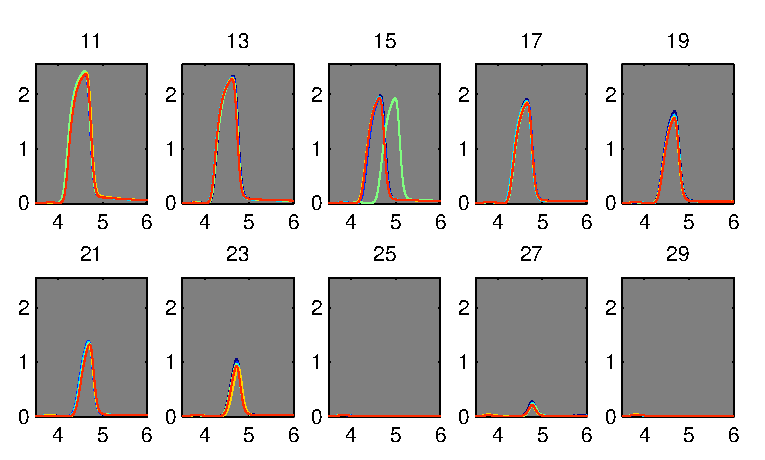
\includegraphics[width=4in]{params_100323_163943.eps}
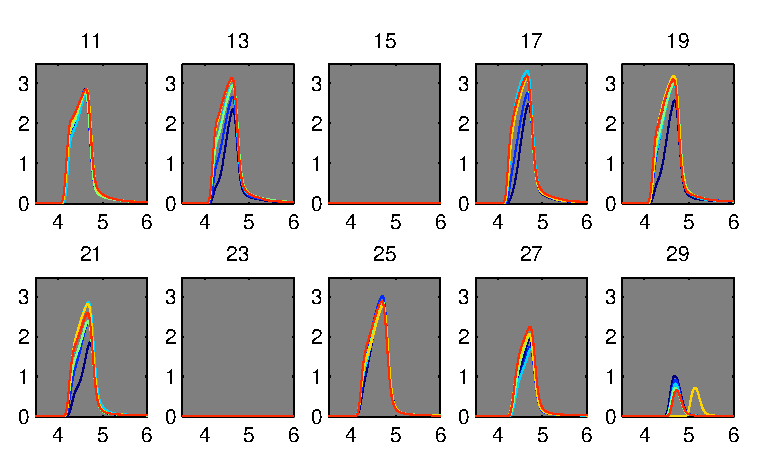
\includegraphics[width=4in]{params_100323_173117.eps}
\caption{Upper two rows is \textbf{params\_100323\_163943}, with check
  valves. Lower two rows is \textbf{params\_100323\_173117} with check
  valves. I later discovered that the response failures were due to
  sticking check-valves.}
\label{fig:one}
\end{figure}


\clearpage
\subsection{24$^{th}$ March 2010}
\label{stickingValves}
Today we try it again. The clean air signal has vastly decreased. I
realised that the check valves were sticking. Passing air through at
800 ml/min does unstick them. However, just playing with the machine
it seems that the PID traces are rather non-stationary. 
\begin{figure}[h]
\centering
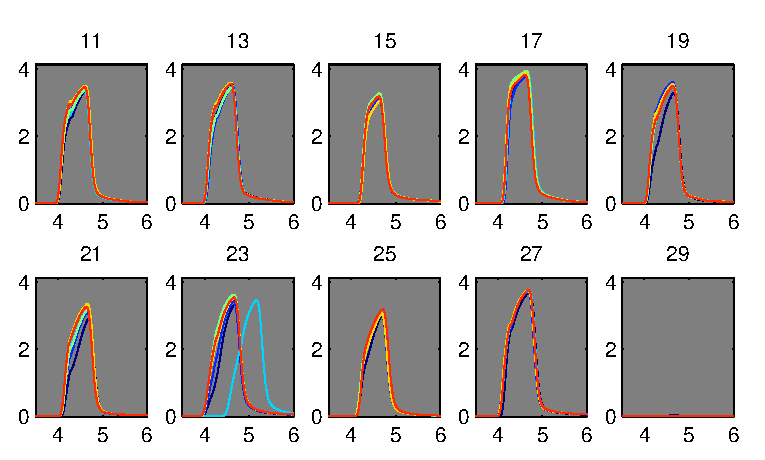
\includegraphics[width=5in]{params_100324_121954.eps}
\caption{\textbf{params\_100324\_121954}:}
\end{figure}
Actually, when I run it for 6 reps it looks pretty good.  The only
issue is that sometimes the odour presentation is delayed by 500 ms
(happened 1/60 in this case). I think this is due to the flow
controller signal being delayed. There is some non-stationarity and I
generally notice a trend for larger responses later on in time.


\begin{figure}
\centering
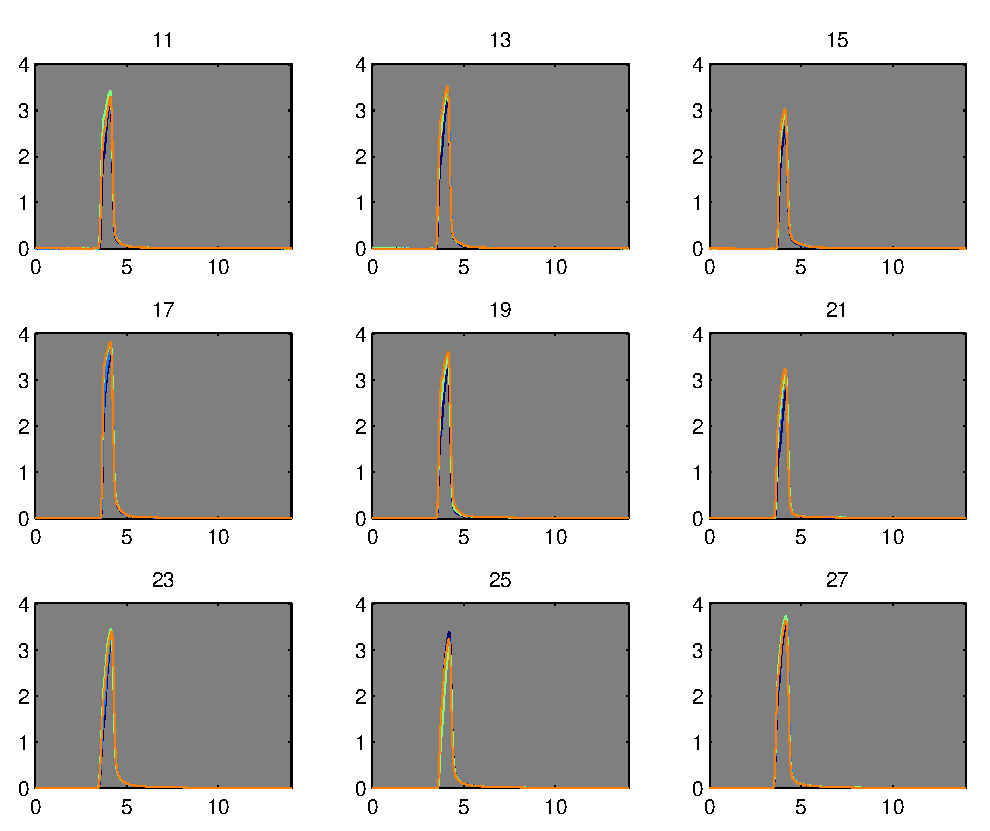
\includegraphics[width=5in]{params_100324_125249.eps}
\caption{\textbf{params\_100324\_125249}:Replace check valve at 25 and
  run again (but with slightly faster ISI and no empty vial). Looks
  better, but the build-up of concentration is a problem. }
\end{figure}


\begin{figure}
\centering
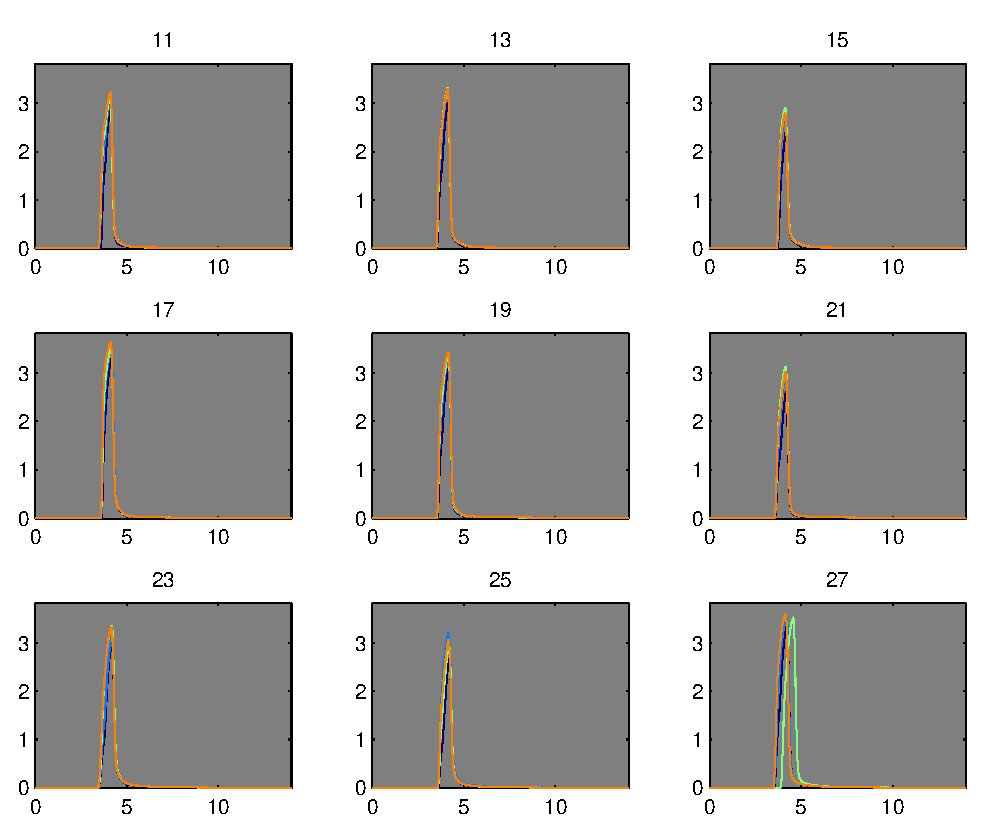
\includegraphics[width=5in]{params_100324_133823.eps}
\caption{\textbf{params\_100324\_133823}:Let's try once more, having
  had the system quiet for 40 minutes.  Still bad. About as bad as
  before.}
\end{figure}

\clearpage
\textbf{Now we apply two changes. }
\begin{enumerate}
\item Keep MFC switched on the whole time and flip between the empty and
odourised vial. The PID signal does go up when I use the empty vial,
but I don't smell anything. 

\item Vial 13 now has a PTFE tube that goes most of the way down to the
liquid. I am experimenting t   o see if this results in more stationary
performance. 
\end{enumerate}
Run two of these with a 20 minute interval (params\_100324\_140642.mat,
params\_100324\_143634.mat). Signals are also smaller. But it's not
clear why that would be. It may be crap building up in the head. 



\begin{figure}
\centering
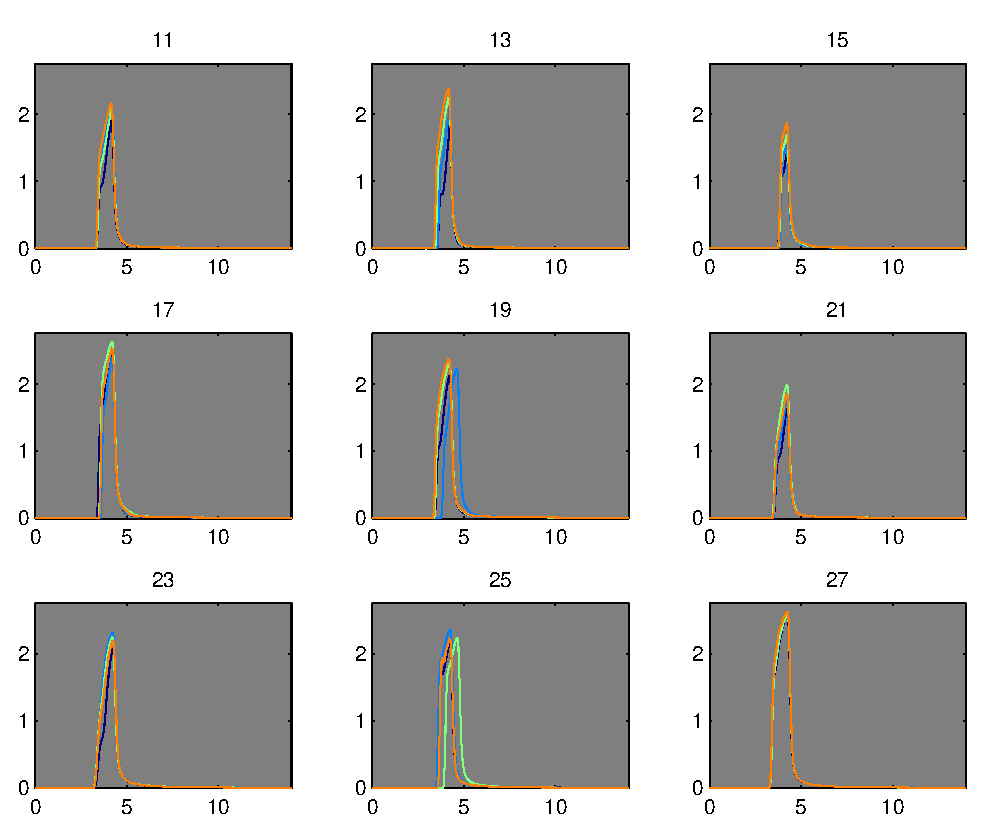
\includegraphics[width=5in]{params_100324_140642.eps}
\caption{\textbf{params\_100324\_140642}:}
\end{figure}


\begin{figure}
\centering
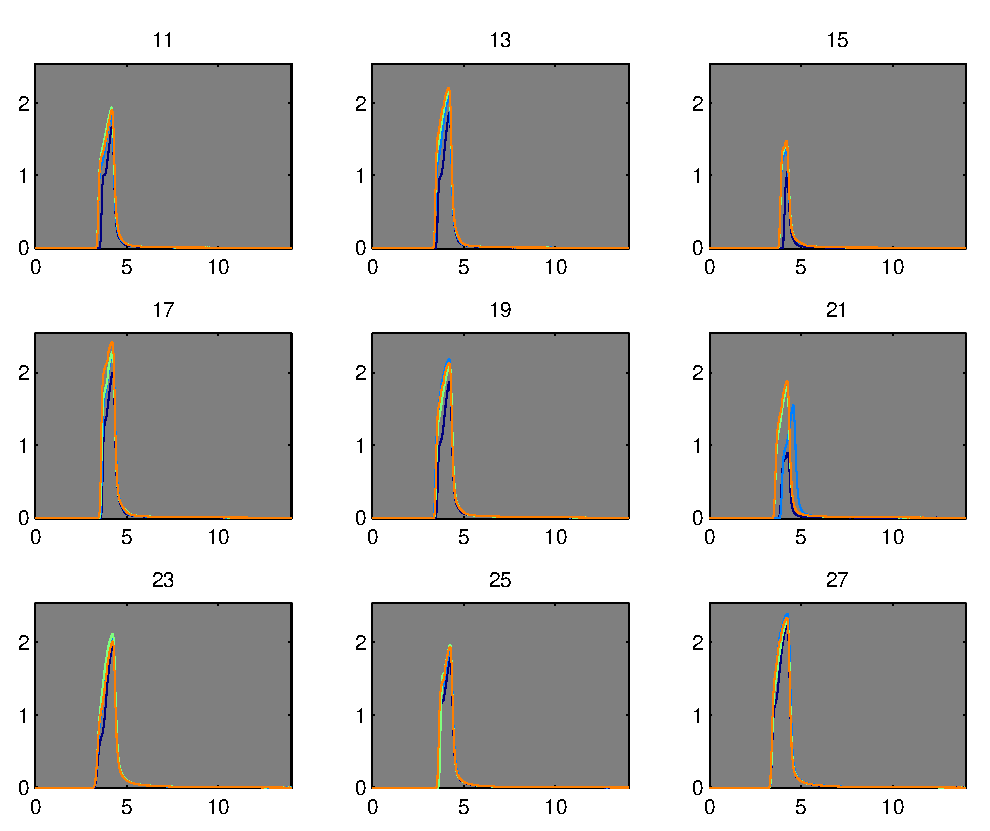
\includegraphics[width=5in]{params_100324_143634.eps}
\caption{\textbf{params\_100324\_143634}:}
\end{figure}
\clearpage
PID went to e-room and was cleaned. params\_100324\_161131.mat Now
it's clipping. That suggests that dirt was the reason why the signal
went down earlier. 

\begin{figure}
\centering
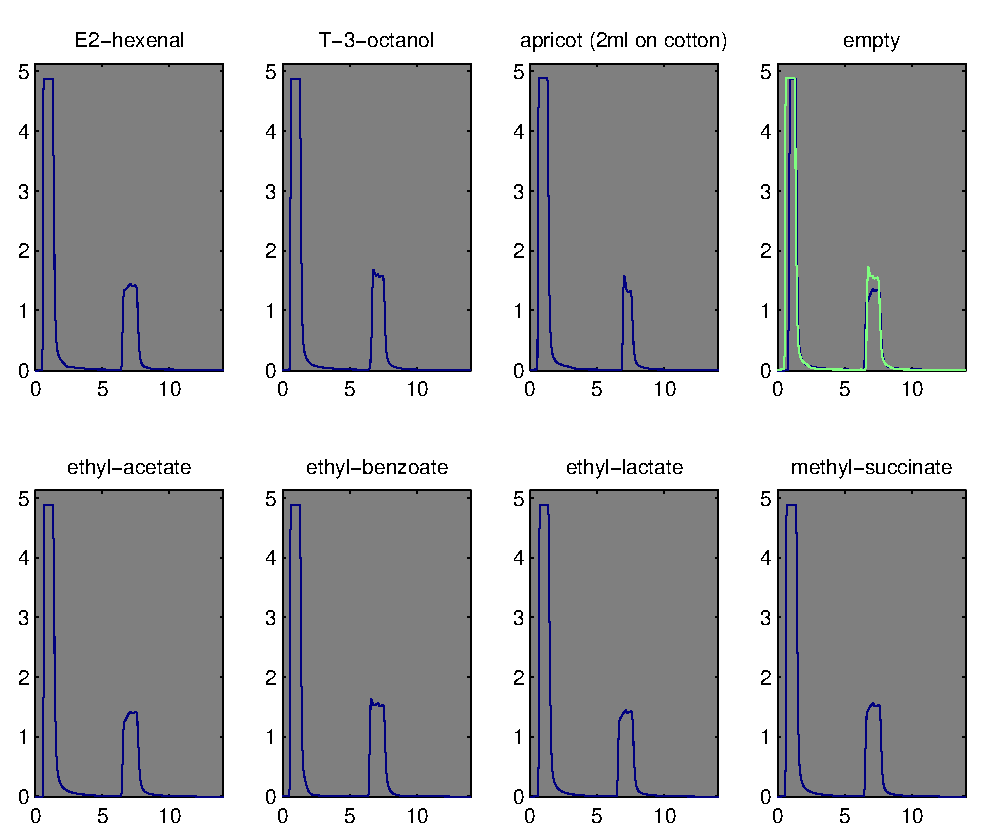
\includegraphics[width=5in]{params_100324_165731.eps}
\caption{\textbf{params\_100324\_165731}:}
\end{figure}

\clearpage
Run it again\ldots
params\_100324\_170457.mat (gain settings are lower)
This time we deliver a 0.5 s pulse at 800 ml/min about 5 s before the
"true" odour pulse. Let's see if this makes things better. Yes, it
does make things better. I'm starting to suspect these weird delays
are due to the check-valves because you see them less with a higher
flow rate. 


\begin{figure}[h]
\centering
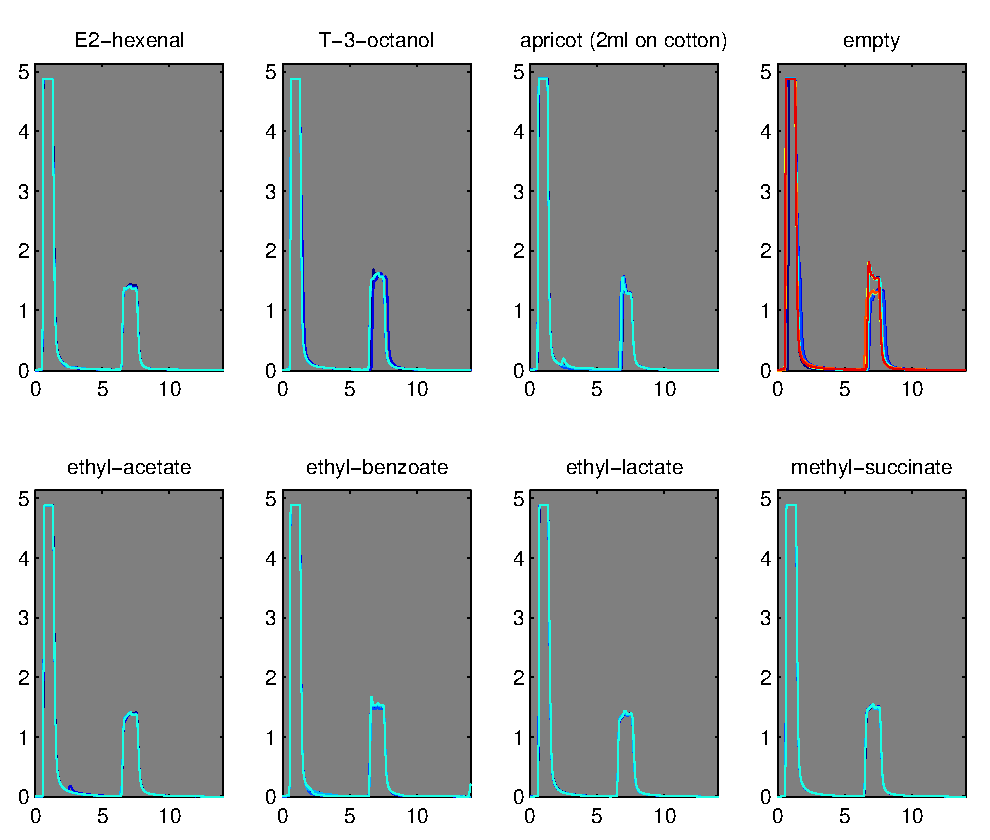
\includegraphics[width=5in]{params_100324_170457.eps}
\caption{\textbf{params\_100324\_170457}:}
\end{figure}




\clearpage
\subsection{25$^{th}$ March 2010}
Set gain to x5 and bubble air through ethanol in tube 13.  Bubbling
air through the ethanol at 200 ml/min doesn't seem to cause crap to
fly around everywhere. This is likely because the flow rate is low and
we're not allowing pressure to build up. The signal is much higher
from this vial but not clipping PID. We run x5 and see if it's
reproducible. See params\_100325\_125504. I don't know why, but vial
27 is producing a much larger signal than the others.

\begin{figure}[h]
\centering 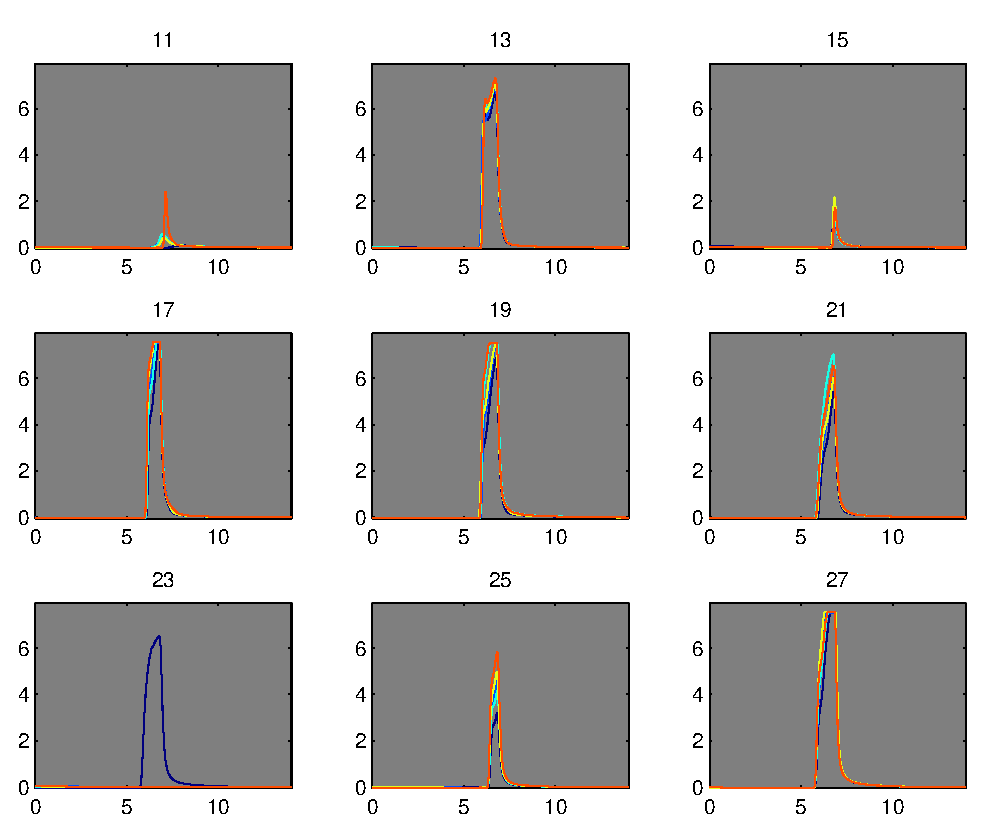
\includegraphics[width=5in]{params_100325_125504.eps}
\caption{\textbf{params\_100325\_125504}:}
\end{figure}


\begin{figure}
\centering
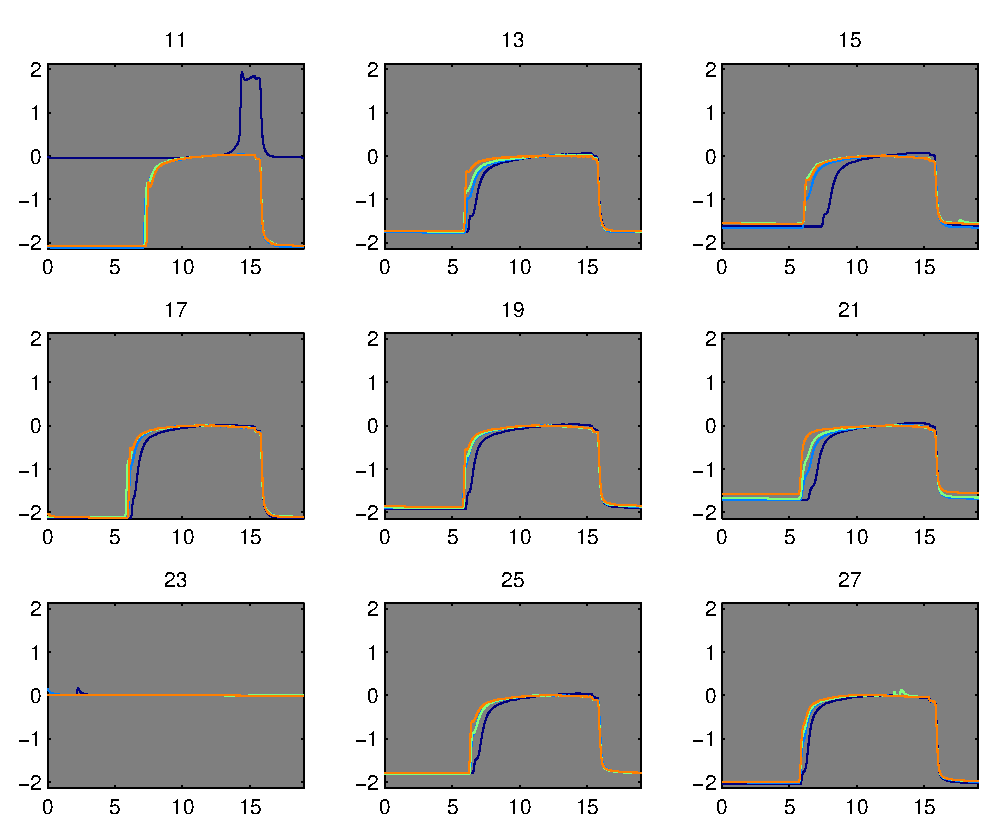
\includegraphics[width=5in]{params_100325_144139.eps}
\caption{\textbf{params\_100325\_144139}:Now run 10 seconds of odour
  through each vial to see how flat the response is. I have set the
  PID gain to 1x, otherwise the signal saturates the amp for some
  vials.  It's too erratic. }
\end{figure}


\begin{figure}
\centering
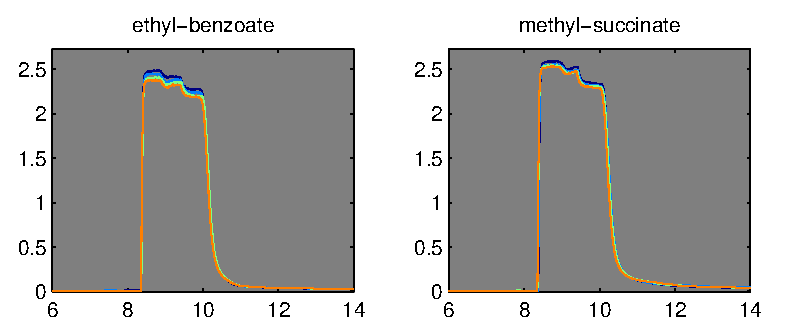
\includegraphics[width=5in]{params_100325_161650.eps}
\caption{\textbf{params\_100325\_161650}: Because the last was too
  erratic I set up the old final valve with just the last pair of
  valves. One is odour one is clean air. The OFF step is brought about
  by the vial switching off so that the whole system cleans out.
  Doesn't look too bad }
\end{figure}


\begin{figure}
\centering
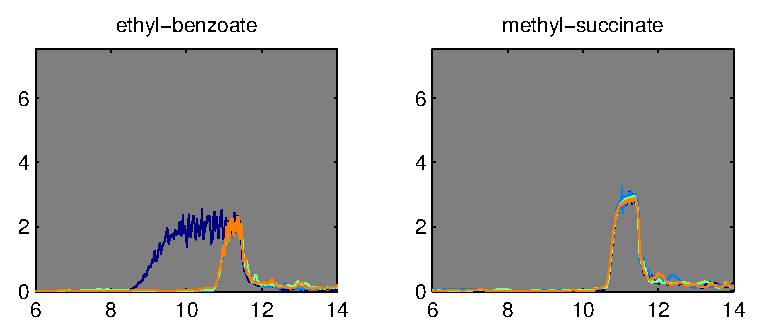
\includegraphics[width=5in]{params_100325_164606.eps}
\caption{\textbf{params\_100325\_164606}: Fiddled with the code a
  bit. Noticed that flow through the vial goes down when we're routing
  it through the valve. Repeated it again and it looks really awful
  but I don't know why.  }
\end{figure}

\clearpage
\subsection{26$^{th}$ March 2010}
Ok ,it looks like the small diameter of the final valves (1/16th inch)
means that the check valves don't open right. 
I have put an old, crappy, check into valve 13 where we're bubbling. 
Bubble at 0.5 L/min for 3 secs then down to 0.2 then present. Also,
I'd bubbled extensively through that vial before for testing. Looks
awesomely good.
\begin{figure}[h]
\centering
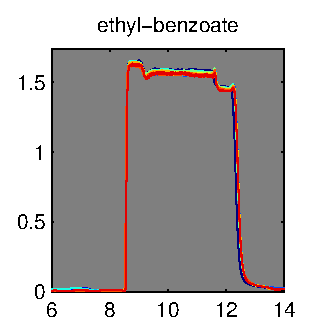
\includegraphics[width=1.5in]{params_100326_131251.eps}
\caption{\textbf{params\_100326\_131251}: Nice\textit{!}}
\label{fig:equilibrated}
\end{figure}


Now wait two hours and run it again: params\_100326\_151344.mat
The first two stimulus presentations are higher than the rest so the
system does take a little time to equilibrate. Wait half an hour and
we get the same problem. params\_100326\_154004.mat
\begin{figure}[h]
\centering
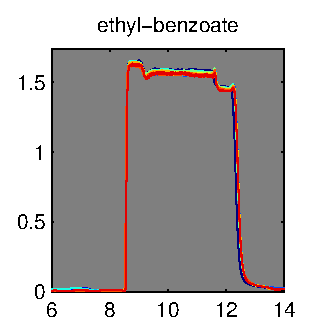
\includegraphics[width=1.1in]{params_100326_131251.eps}
\includegraphics[width=1.1in]{params_100326_151344.eps}
\includegraphics[width=1.1in]{params_100326_154004.eps}
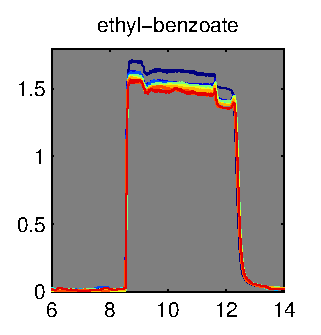
\includegraphics[width=1.1in]{params_100326_161720.eps}
\caption{\textbf{params\_100326\_131251; params\_100326\_151344;
    params\_100326\_154004; params\_100326\_161720}:}
\end{figure}







\begin{figure}
\centering
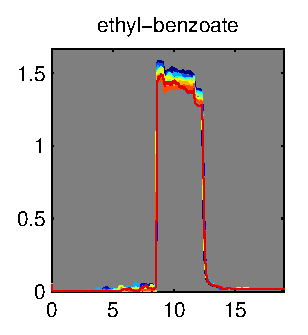
\includegraphics[width=1.5in]{params_100326_162803.eps}
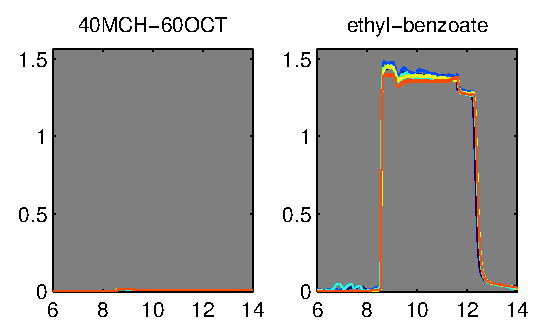
\includegraphics[width=3in]{params_100326_163150.eps}
\caption{\textbf{params\_100326\_162803} \&
  \textbf{params\_100326\_163150}: I increased the time over
  which we bubble at a higher rate and that has increased variance. }
\end{figure}

\begin{figure}
\centering
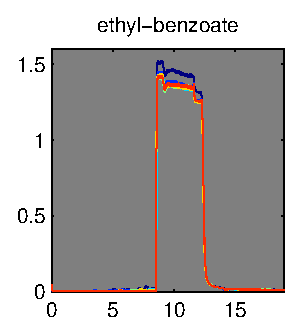
\includegraphics[width=2.5in]{params_100326_163630.eps}
\caption{\textbf{params\_100326\_163630}:}
\end{figure}


\begin{figure}
\centering
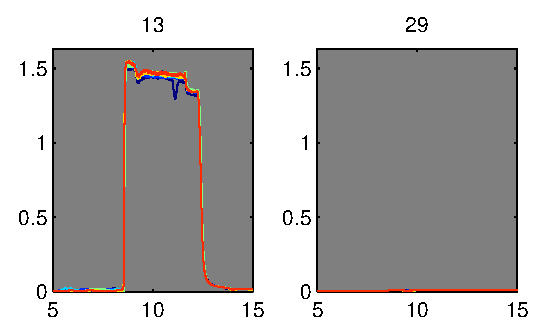
\includegraphics[width=4in]{params_100326_165043.eps}
\caption{\textbf{params\_100326\_165043}:Looking better now that I set
  pre-presentation bubbling to 0.4 }
\end{figure}


\clearpage
Fill V13 1/10 with ethanol and run it 15 times to see what it looks
like. Eeek. It clearly hasn't equilibrated yet. I also forgot to vortex it. 
params\_100326\_171154.mat
First rep was at 1x gain. 


Will vortex and try again.  params\_100326\_172130.mat
That's no better. It's still going down. 

longer ISI may have improved things. I wonder if with a diluted odour
I shouldn't be bubbling for as long. Try that. 
load params\_100326\_180042.mat

\begin{figure}[h]
\centering
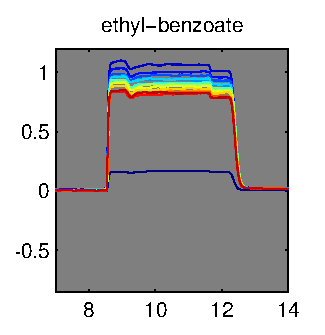
\includegraphics[width=2in]{params_100326_171154.eps}
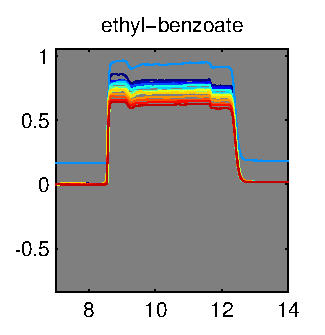
\includegraphics[width=2in]{params_100326_172130.eps}
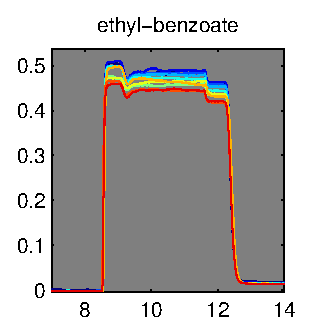
\includegraphics[width=2in]{params_100326_180042.eps}
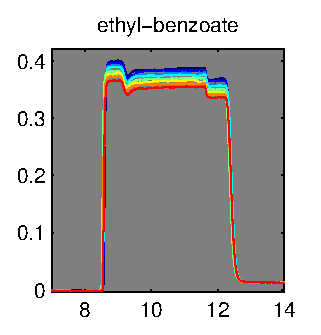
\includegraphics[width=2in]{params_100326_181209.eps}
\caption{\textbf{params\_100326\_171154},
  \textbf{params\_100326\_172130},
 \textbf{params\_100326\_180042}, \textbf{params\_100326\_181209}.}
\end{figure}
Looking at the PID trace, it seems that 1s at 0.4 ml/min is enough to
increase the odour concentration to where it ought to be. So we do 1s
at 0.4 then go down to 0.25 (which is where most of today has been
done) to present the odour to the fly. 

The concentration is just more stable when we're dealing with pure
odour. As soon as you dilute it then it starts to run down. This is
because the vapour pressure decreases. With pure odour that can't
happen. Go back to pure odour, I think!





\clearpage
\subsection{27$^{th}$ March 2010}
Could it be that diluting at 1:1000 will improve the problem?
params\_100327\_154706.mat
params\_100327\_160249.mat
No, it still goes down at every presentation. What's worse is that we see the
higher level of the odour valve to be more a problem. I'll pull apart
the tubing there and see if I can clean it. 

One last possibility: What if it takes it overnight to equilibrate?
Try the 1:10 again. No, quite the opposite: params\_100327\_161423.mat
\begin{figure}[h]
\centering
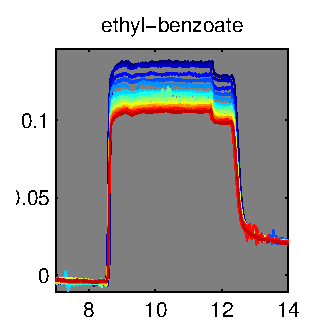
\includegraphics[width=1.5in]{params_100327_154706.eps}
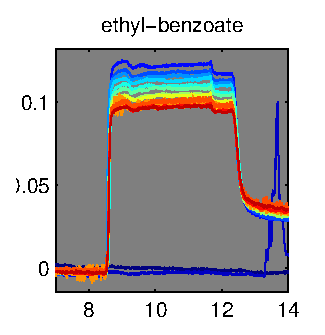
\includegraphics[width=1.5in]{params_100327_160249.eps}
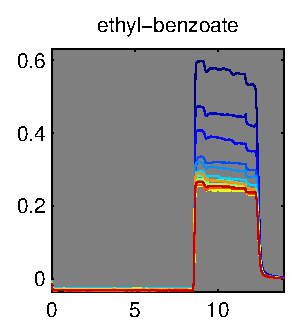
\includegraphics[width=1.5in]{params_100327_161423.eps}
\caption{In order: \textbf{params\_100327\_154706},
  \textbf{params\_100327\_160249}, \textbf{params\_100327\_161423}.}
\end{figure}


\clearpage
\subsection{28$^{th}$ March 2010}
I had noticed that the stream from the vials had a higher resting PID
value than the clean air stream. Vial 13 was attached to an old style
valve and a 1/1000 ethanol vial. When I replaced this vial with one
containing an essential oil on cotton wool, the basal PID signal
decreased. It looks like this higher signal may simply be due to the
odours and can be fixed by the fancy Parker valves. Changing the clean
air vial didn't alter anything and placing a clean air vial into the
clean air stream didn't help either. 

Today we won't use the final valve because I'm cleaning the
Y. Instead, we put the PID directly onto the end of the tube coming
from the odour delivery system. 

I then present odour through the essential oil vial so we can evaluate
it for stationarity: params\_100328\_152704 \& params\_100328\_153325.
We still see concentration drops on each stimulus presentation.   

\begin{figure}[h]
\centering
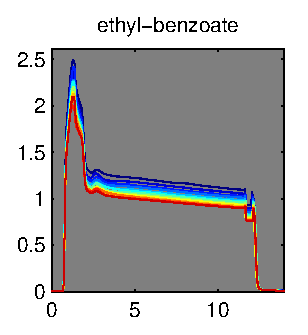
\includegraphics[width=1.5in]{params_100328_152704.eps}
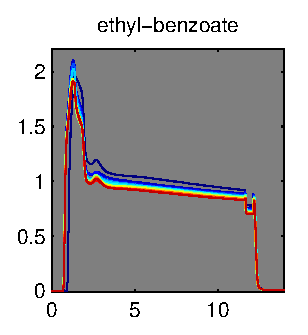
\includegraphics[width=1.5in]{params_100328_153325.eps}
\caption{\textbf{params\_100328\_152704}, \textbf{params\_100328\_153325}}
\end{figure}

\clearpage

Now try with the 70/30 OCT/MCH mixture. 
This also goes down. It looks like there'll be no way of avoiding this
unless we use saturated vapour. I think that for non-saturated vapour,
params\_100328\_155935.mat \& params\_100328\_160854.mat
I'm probably forcing through too much air. We'd need to bubble
initially so that we get rid of high-concentration head space. But
then I could probably bubble at just 0.25ml/min for 7 s or so. Try
this next\ldots

It's not run out: params\_100328\_161932.mat


I put the pure ethanol vial back and present a few pulses to check it
out again. Is it really better than the diluted odours?
YES: params\_100328\_162845.mat

Ok... So can I shove a 1ml/min pulse into the stream and pick it up??
No. It looks like the carrier creates pressure which stops odour from
entering the stream. If the difference between the streams is more
than about 1/10, we get a problem. 


\begin{figure}[h]
\centering
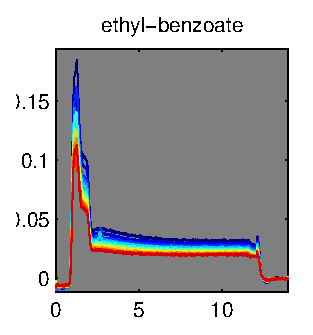
\includegraphics[width=2in]{params_100328_155935.eps}
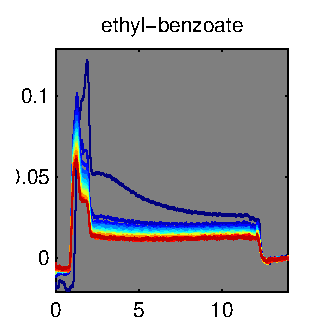
\includegraphics[width=2in]{params_100328_160854.eps}
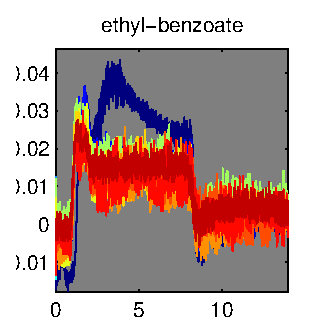
\includegraphics[width=2in]{params_100328_161932.eps}
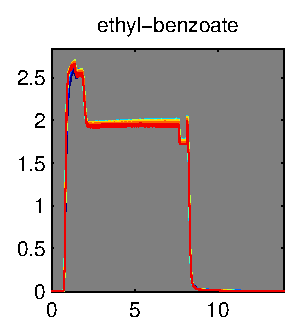
\includegraphics[width=2in]{params_100328_162845.eps}
\caption{\textbf{params\_100328\_155935},
  \textbf{params\_100328\_160854}, \textbf{params\_100328\_161932},
\textbf{params\_100328\_162845}.}
\end{figure}


\clearpage
\subsection{29$^{th}$ March 2010}
We have decided to run the oct/mch experiment using
dilutions. Firstly, I will run ethanol though all vials and choose 6
which are best matched. Secondly, then I equalise the intensity of the
MCH and Octanol with the T-maze. I will also see if using a large
volume of liquid works better than a small volume. I.e. a more stable
trace can be obtained this way. 

Ok. We try to present each 5 times. This is 50 reps but the data
acquisition seems to have halted at 34, for some odd reason. Try to
work out why. Ah! It's because I started PV!  Before each of the
following I'm bubbling at 0.5 ml/min for 10 s through each vial in
turn and then beginning the acquisition. 


\begin{figure}[h]
\centering
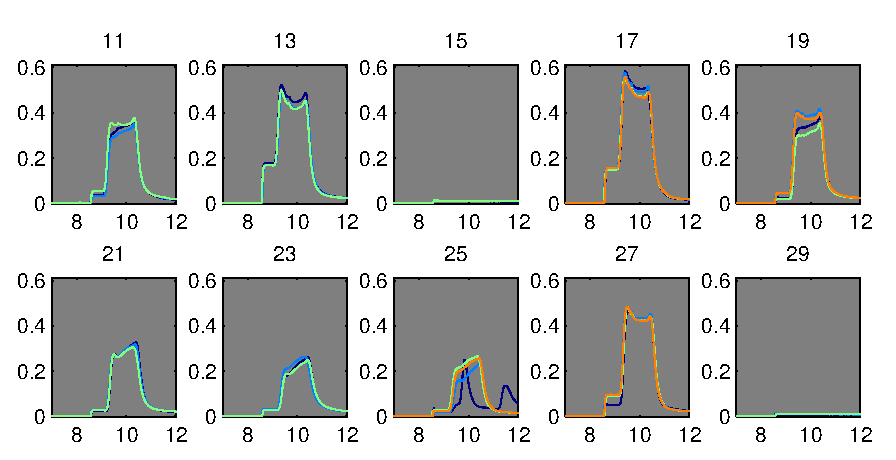
\includegraphics[width=5in]{params_100329_115622.eps}
\caption{\textbf{params\_100329\_115622}:}
\end{figure}


I'm having troubling getting valve 15 to open: params\_100329\_122851.mat
Will try blasting with 0.4 ml/min for 2 seconds before dropping to
0.25. If that doesn't work, I'll just see if I can do it all at
.25. Probably have to anyway, since I think we'll need a high flow
rate to get the t-maze concentrations. 
No, this didn't work either: params\_100329\_132054.mat


\begin{figure}[h]
\centering
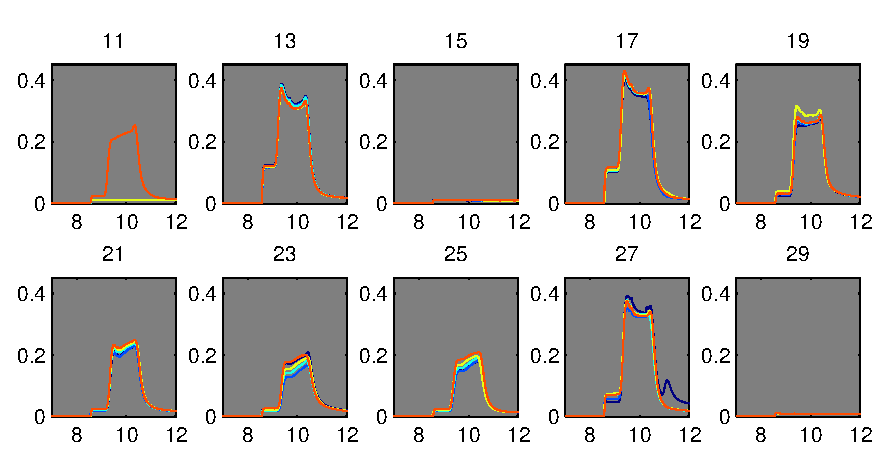
\includegraphics[width=4in]{params_100329_122851.eps}
\caption{\textbf{params\_100329\_122851}:}
\end{figure}


\begin{figure}
\centering
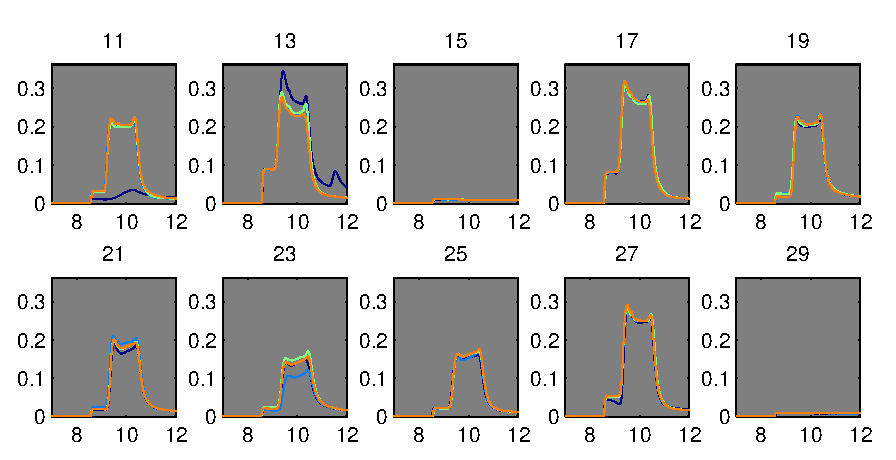
\includegraphics[width=4in]{params_100329_132054.eps}
\caption{\textbf{params\_100329\_132054}:}
\end{figure}

\clearpage
Ok:
So I will try presenting the odours at 0.4 ml/min
It's nicer and more consistent at 0.4. 
params\_100329\_134328

\begin{figure}[h]
\centering
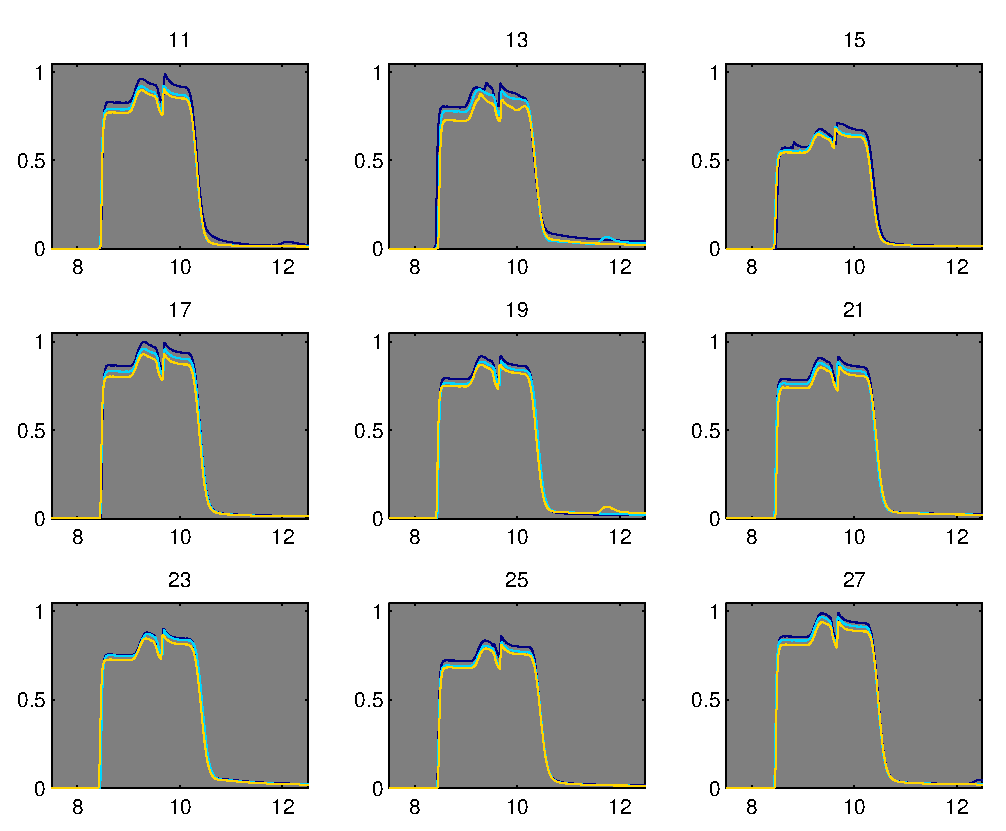
\includegraphics[width=5in]{params_100329_134328.eps}
\caption{\textbf{params\_100329\_134328}:}
\end{figure}


\clearpage
I'll run more at 0.5 but will only run those vials that look fairly
similar to each other: 11,13,19,21,23,27
params\_100329\_140034: ok, but 27 is too high. Replace it with 17 and
see how that goes
params\_100329\_143349.mat

It's not as stable as it was before. I've not been bubbling. So repeat
it but bubble this time. 

\begin{figure}[h]
\centering
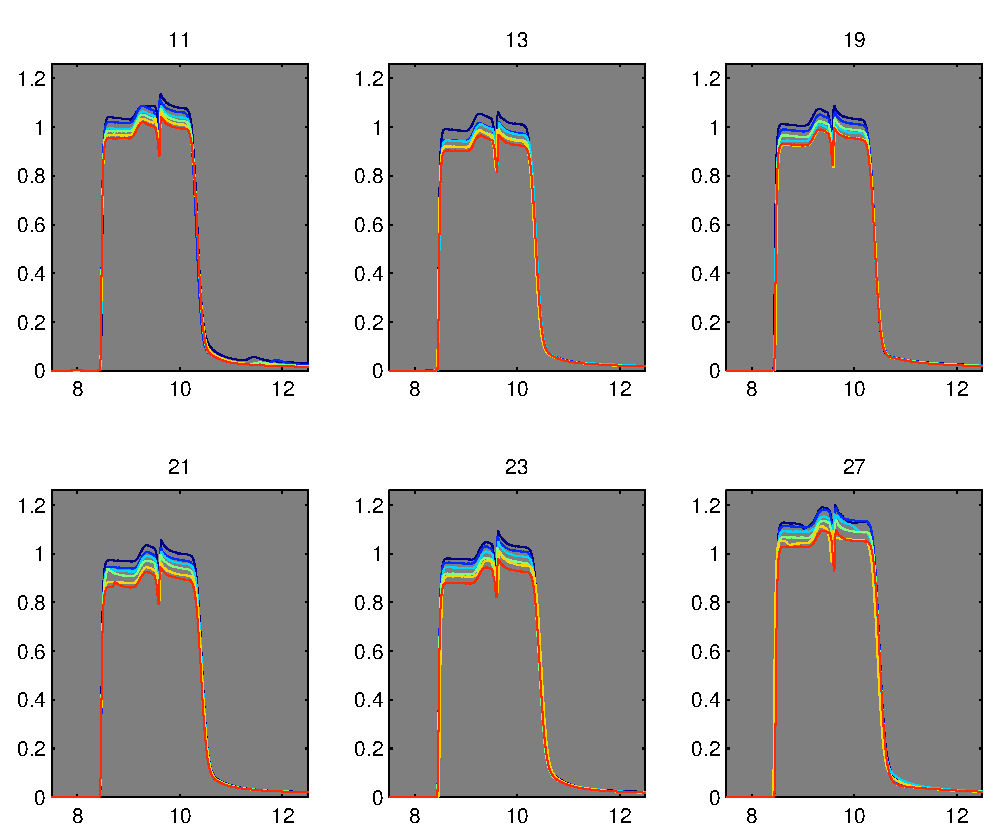
\includegraphics[width=3.4in]{params_100329_140034.eps}
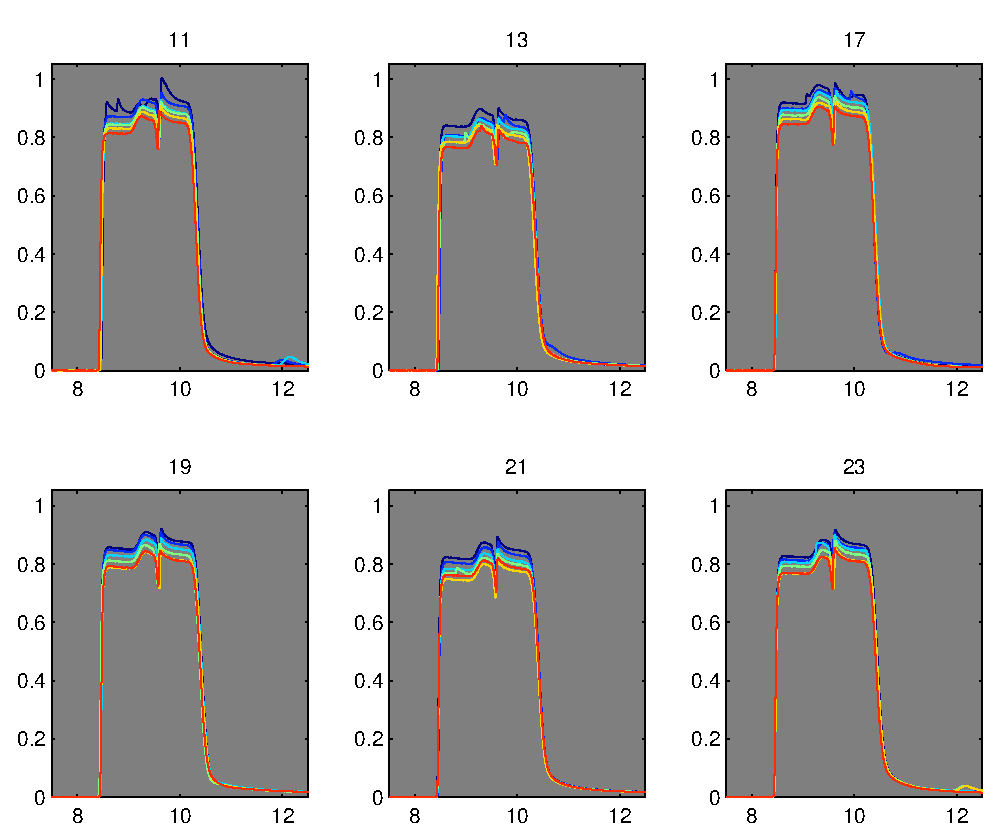
\includegraphics[width=3.4in]{params_100329_143349.eps}
\caption{\textbf{params\_100329\_140034}, params\_100329\_143349}
\end{figure}

params\_100329\_163902.mat Still goes down over time. 
It's also lower than the values we got without bubbling. Argh!

\begin{figure}[h]
\centering
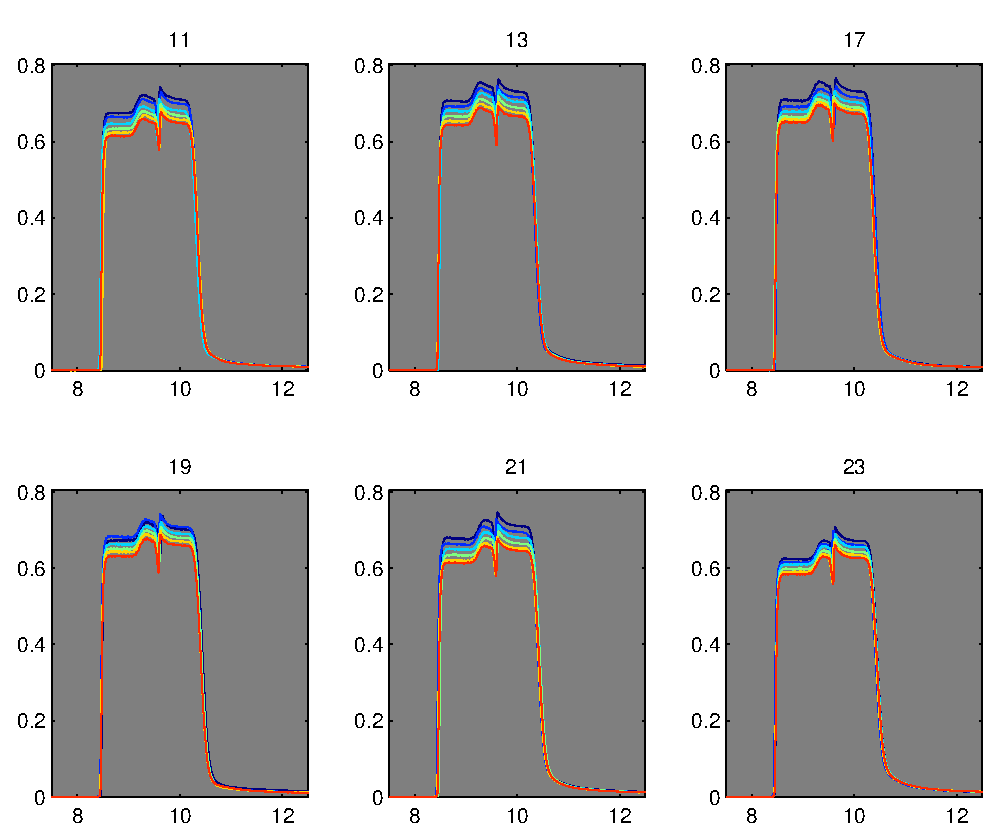
\includegraphics[width=4in]{params_100329_163902.eps}
\caption{\textbf{params\_100329\_163902}:}
\end{figure}

Run it once more because I want to see whether the signal becomes
lower than the last: params\_100329\_172731.mat
Shit, the signal is going down.  For all vials. 
Let's present x5 from 17 and another vial which hasn't been much used
recently: 27


\begin{figure}[h]
\centering
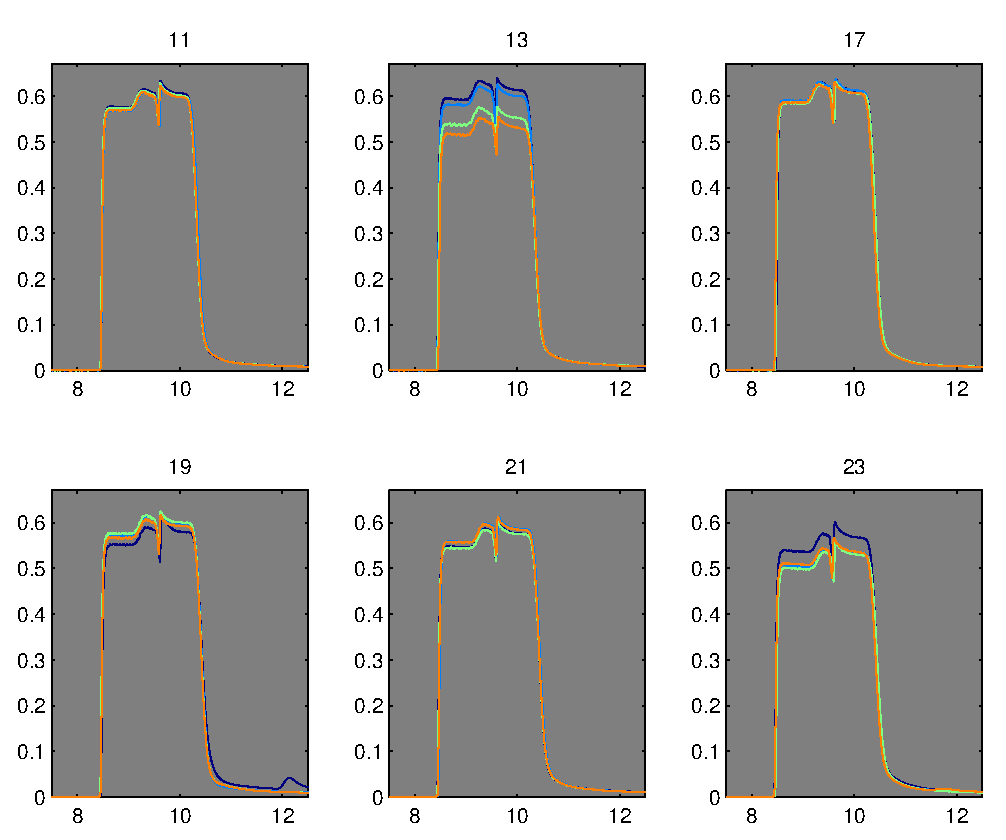
\includegraphics[width=4in]{params_100329_172731.eps}
\caption{\textbf{params\_100329\_172731}:}
\end{figure}

\clearpage
Everything's going down (params\_100329\_175103.mat) since 27, which
I've not been using, is also low now. I think it's the PID....
Let's clean it and try again

\begin{figure}[h]
\centering
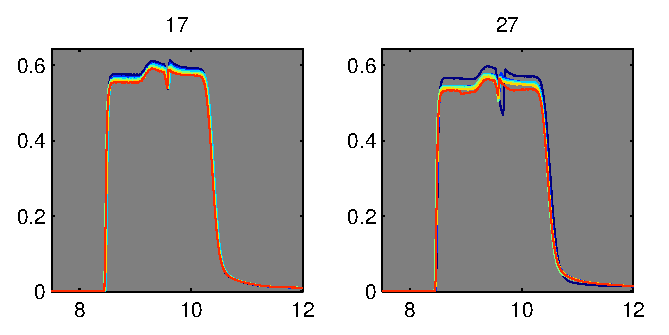
\includegraphics[width=4in]{params_100329_175103.eps}
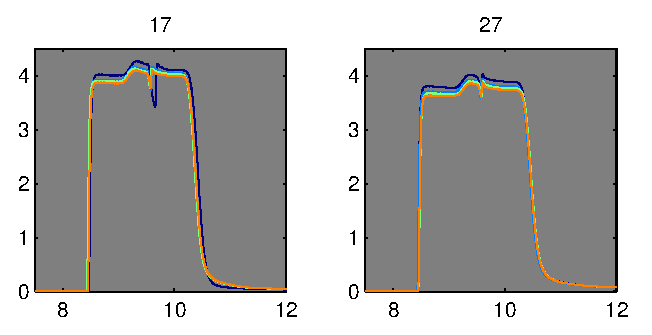
\includegraphics[width=4in]{params_100329_181309.eps}
\caption{\textbf{params\_100329\_175103}: Everything's going down
  since valve 27, which I've not been using, is also low now. I think
  it's the PID....  Let's clean it and try
  again. \textbf{params\_100329\_181309}:
Yeah, fuck. That was it! So maybe the Oct/MCH wasn't really running
down after all? This wasn't flushed before recording. }
\end{figure}



\begin{figure}
\centering
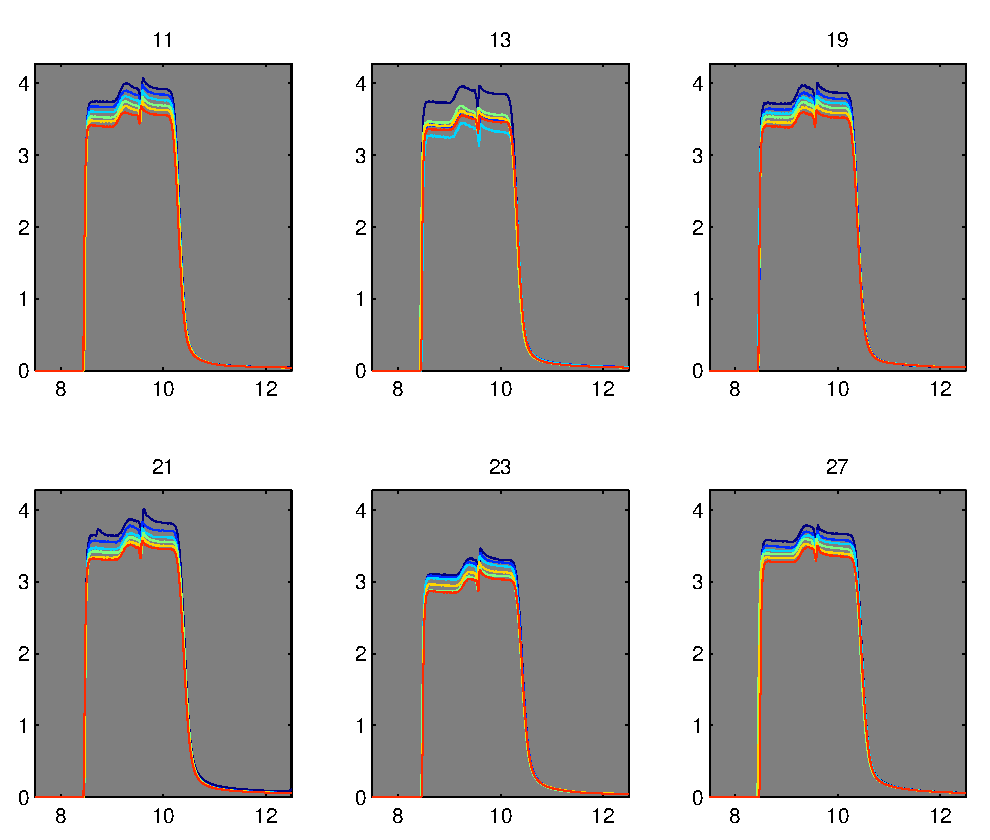
\includegraphics[width=5in]{params_100329_182227.eps}
\caption{\textbf{params\_100329\_182227}:Let's re-run what we were
  doing before. \textit{I really don't know why I got some
    consistently high readings before and not now. No idea. But it
    does look like the decrease in sensitivity is due to the PID. At
    least in this case. } }
\end{figure}

I'll just do some MCH...
Set PID to x1 and suction to low
Set flow through the vial to 500 ml/min and stick it into \#27 with the
old (crappy) check valve and bubble. The MCH was freshly made today. 
Sod. The gain had to be at x10, because that's what we used for
e-room. Do it again\ldots params\_100329\_185604.mat
params\_100329\_184718.mat

\begin{figure}[h]
\centering
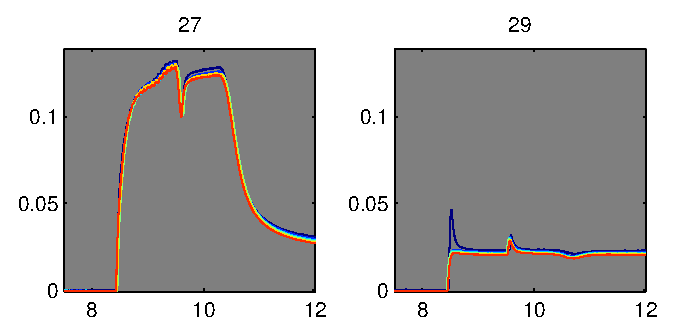
\includegraphics[width=4in]{params_100329_184718.eps}
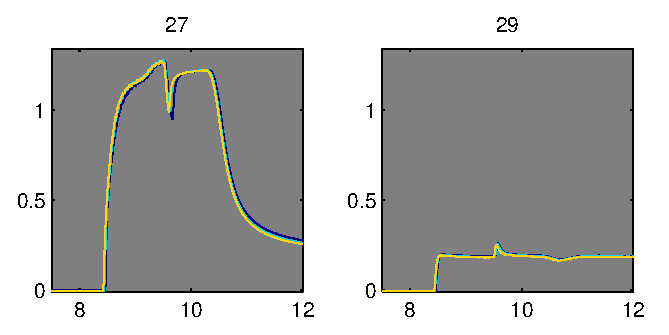
\includegraphics[width=4in]{params_100329_185604.eps}
\caption{Top: \textbf{params\_100329\_184718}, wrong gain. Bottom:
  \textbf{params\_100329\_185604}, with the correct gain. This is too
  low and we're getting a valve switching artifact. I suspect because
  of the high flow rate.  }
\end{figure}







\clearpage
\subsection{30$^{th}$ March 2010}
Clean PID again using air from the wall. Dropped the bulb, but it's
not cracked and the PID lit up straight away. Flow set to low.
\begin{figure}[h]
\centering
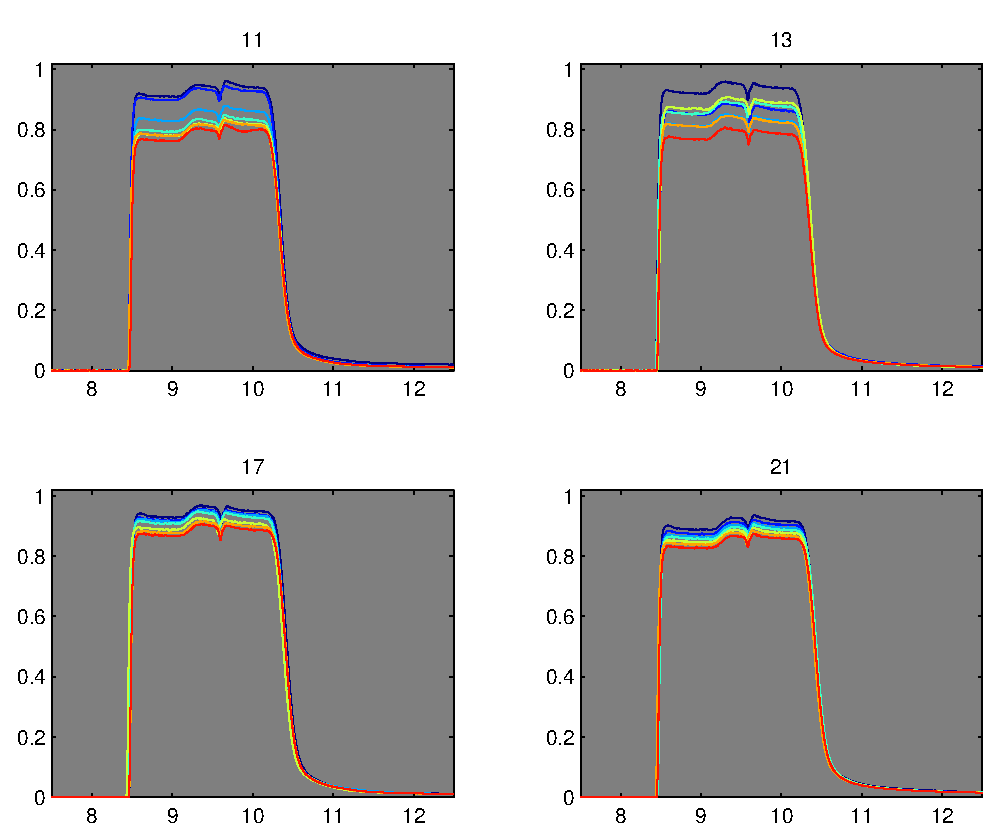
\includegraphics[width=4in]{params_100330_115524.eps}
\caption{\textbf{params\_100330\_115524}:  Test with ethanol from 4
of vials. 6 reps each. Bubbling through each. Odour flow is 0.5/0.5
\textit{why} does it now look so bad? It was stationary before! }
\end{figure}

\begin{figure}[h]
\centering
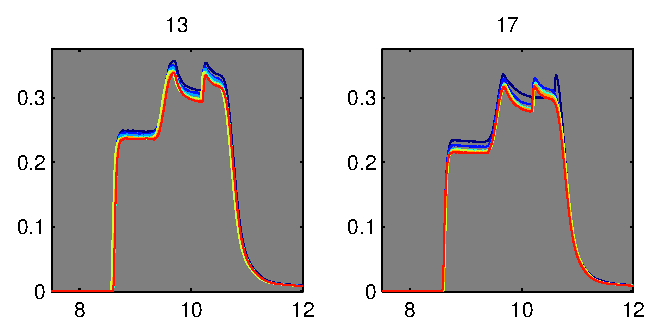
\includegraphics[width=4in]{params_100330_121140.eps}
\includegraphics[width=4in]{params_100330_123018.eps}
\caption{\textbf{params\_100330\_121140}: Try dropping down to 0.25
  ml/min. Yeah\ldots that looks better. 
And again at 0.2: params\_100330\_123018. }
\end{figure}




\begin{figure}[h]
\centering
\includegraphics[width=4in]{params_100330_162733.eps}
\caption{\textbf{params\_100330\_162733}:PID was running all
  afternoon. Cleaned it again. Wow, the signal went up. This thing
  needs regular cleaning. I am running it again with the flow at 0.2
  and total flow at 1 (the previous two in the preceding fig were
  actually at a higher total flow).  }
\end{figure}

I played around with the relative flow rates at the vials and found
that the signal at the PID is lower if the ratio of carrier to odour
is not 50/50. i.e. 200 ml/min odour and 200 ml/min air is a stronger
response than 400 ml/min odour. I do another run, therefore, with the
valves we'll want to use and with 0.35 l/min going through both
carrier and odour. 

\begin{figure}[h]
\centering
\includegraphics[width=4in]{params_100330_174954.eps}
\caption{\textbf{params\_100330\_174954}: \#27 is actually an MCH vial
which we won't end up using. The signal goes down over time but this
may be because of the flushing procedure. It flushes through 0.5 l/min
but the odour is less than that. Perhaps it takes a while to settle. I
therefore run it again, below, without the flushing. }
\end{figure}

\begin{figure}[h]
\centering
\includegraphics[width=4in]{params_100330_180600.eps}
\includegraphics[width=4in]{params_100330_182240.eps}
\caption{\textbf{params\_100330\_180600}: Still goes down. How about
  we flush at the same rate that we'll be presenting at? Also, clean
  the PID again. The result of this is in the bottom two rows:
  \textbf{params\_100330\_182240}: now in some vials it's going up. }
\end{figure}

\begin{figure}[h]
\centering
\includegraphics[width=4in]{params_100330_185432.eps}
\caption{Deliver once more with no PID, see if we can equalise
  everything further. Then record:
  \textbf{params\_100330\_185432}. This is looking better. So it takes
  it a looong time to equilibrate and it's a BAD idea to be running
  air through at different odour concentrations. }
\end{figure}

So now, all I need to do is equalise the concentrations. First we
present a load of stuff through \#27, since we weren't doing this and
we need 6 vials. 

\begin{figure}[h]
\centering
\includegraphics[width=4in]{params_100330_192526.eps}
\includegraphics[width=4in]{params_100330_194547.eps}
\caption{Top: \textbf{params\_100330\_192526}. Clean the PID and
  repeat Bottom \textbf{params\_100330\_194547}. Equilibrating takes a
loong time!}
\end{figure}


\clearpage
\subsection{31$^{th}$ March 2010}
Blast air through all the check valves. Now flush the 7 valves we'll
use for 15 s each. Then present stimuli. Do everything at 0.35 ml/min
Ooh. They look totally different. Very smooth traces now. 

\begin{figure}[h]
\centering
\includegraphics[width=4in]{params_100331_110932.eps}
\caption{\textbf{params\_100331\_110932}: This is a disaster. The
  final valve is switching at 8s then nothing happens until 2 seconds
  later. 11 is way bigger than the others and 13 doesn't respond at
  all. }
\end{figure}
Ohh! Check valve 13 was disconnected so the system wasn't
pressurised. 


\begin{figure}[h]
\centering
\includegraphics[width=4in]{params_100331_115521.eps}
\caption{\textbf{params\_100331\_115521}:}
\end{figure}

Replace the check valve in \#23 and then flush/run for 3 reps. 
\begin{figure}[h]
\centering
\includegraphics[width=4in]{params_100331_131419.eps}
\caption{\textbf{params\_100331\_131419}: It's \textit{still} lower.}
\end{figure}


\begin{figure}[h]
\centering
\includegraphics[width=4in]{params_100331_132312.eps}
\caption{\textbf{params\_100331\_132312}: We can get much nicer curves that are closer to 1s in duration if we
switch the vial \textbf{off} 100~ms before the odour valve opens. The
stimulus duration parameter doesn't do anything in the delivery code
in this context. }
\end{figure}

Why are the signals from different vials of different strength?
I'll check the flow rates from all the vials. In the process of doing
this, I found a bug in the code: when the system was being asked to go
to valve 29, it was failing to do so. Instead it just shut all flow to
the valves. I am therefore now running it again, with the bug
corrected. Ok, so the flows. They're very similar:

\begin{tabular}{|l|l|}
\hline
Valve & flow \\
\hline
29&0.95\\
27&0.93\\
25&0.95\\
23&0.94\\
21&0.93\\
19&0.93\\
17&0.90\\
15&0.96\\
13&0.91\\
11&0.96\\
\hline
\end{tabular}
This was measured as follows: Set the carrier flow to 1 l/min. The
flow meter does indeed register that this is at 1 l/min. The odd thing
is that if I set the vials to be 1 l/min, I only get 0.5
l/min. \textbf{Hmmm. Is there a leak or something I don't understand.}
The flows seem additive when both controllers are on. When I measure
the flow at the odour MFC, I get about 950 ml/min. The carrier is
about 1050 ml/min. So maybe I should service these things? When I
measure after valve 31, I get about 800 or 900 ml/min. So There must
be a leak up there. I'll ignore it for this week, since I need to get
data. But when I build the new system, \textit{the first thing to
  check for is that the flows add up correctly}. So build the system
with empty vials first.  Regardless, I ask what flow through the vial
do I need to achieve a total flow of 1,500 ml/min. These are the
values in the table. They appear very similar for most vials. I choose
the vials which are most similar and run the thing again. Let's see
what it looks like now.

\begin{figure}[h]
\centering
\includegraphics[width=4in]{params_100331_140949.eps}
\caption{\textbf{params\_100331\_140949}: Don't know why 23 and 15
  look so bad. Only they're similar to each other. I say I go ahead
  with oct and mch in these two then the rest of the odours can be
  other vials. It's worth noting that the stimulus latency is supposed
to be at 8 s. It's clearly not. So that is worth fixing.}
\end{figure}


So first I replace all vials with empties (wide bore outlet tube) and
flush: pump 1 l/min through each vial for 15 s each. Keep doing this
whilst I prepare the odourants. \textbf{Ah!} I found that some vials smelled
quite strongly of odour. At first I thought it was that the tubes
hadn't been cleaned properly downstairs. The tubes are now being
boiled in water and ethanol. But then I discovered that the inlet
check valves smelled quite strongly. So now those a boiling too. I
changed most of them (apart from tubes 21,23,and 25, because these
were the least bad and I've run out of untainted check valves). There
is still some signal and I'm worried that it's coming from the
valve. There's really nothing I can do now. I'll just keep flushing
and use the same vials I had originally planned. 


\subsubsection{Let's try to do a recording}
I'll begin by shoving 10 ml of the 1.5:1000 MCH into V23 and recording
10 reps of that (no flushing). PID gain is x10 and the suction rate is
on low (900 ml/min). These were the settings used for measuring the
odour concentrations in the RoboTrainer (params\_100331\_161748).  Now
clean the PID and do that again (params\_100331\_164630).

\begin{figure}[h]
\centering
\includegraphics[width=4in]{params_100331_161748.eps}
\includegraphics[width=4in]{params_100331_164630.eps}
\caption{Top row: \textbf{params\_100331\_161748}; bottom row:
  \textbf{params\_100331\_164630}. The lower recording when I'd
  cleaned the PID is so much bigger\textit{!} I really think that a
  (large) part of the decrease that we see in the response could be
  due to the PID and not true reduction in concentration. }
\end{figure}

This MCH vial has been used in other recordings over the last few days
(see above). So how much of it has \textit{really} gone down? To
answer this, we clean the PID again and replace the MCH with new
stuff. Now record. 
\begin{figure}[h]
\centering
\includegraphics[width=4in]{params_100331_172029.eps}
\caption{\textbf{params\_100331\_172029}: Great. That's all I
  needed. Now the signal's gone down. }
\end{figure}


The PID response appears to be very weak. I don't trust it. Even with
the nozzle inside the vial's head-space the signal is weak. I wonder
if maybe the bulb is damaged and has sprung a leak? I want to do the
experiment. So sod it. I'll just fill it all up with the T-maze stuff
and go for it. Actually, later I read the manual and realised that the
bulbs can be cleaned with methanol. Did this and the signal has now
shot up. 

\begin{figure}[h]
\centering
\includegraphics[width=4in]{params_100331_195540.eps}
\caption{\textbf{params\_100331\_195540}: OK! we're back in
  business. It was just a lamp clean!}
\end{figure}


\subsubsection{1$^{st}$ April}

\begin{figure}[h]
\centering
\includegraphics[width=4in]{params_100401_143200.eps}
\caption{\textbf{params\_100401\_143200}: Re-insert the odours. The
  signals are about half the size they were yesterday. I obviously
  can't be sure to what degree this is due to the PID. }
\end{figure}


I haven't had much luck today. Very weak responses. Could it be the
homozygous flies or something else? Replace the odours with 1:100 and
1.5:100 dilutions of Octanol and MCH respectively. Vials 15 and 19
aren't opening... ARgh.
converting structure to object

\begin{figure}[h]
\centering
\includegraphics[width=4in]{params_100401_210513.eps}
\caption{\textbf{params\_100401\_210513}: Ignore the first few reps. }
\end{figure}



\subsubsection{Continuing to diagnose the machine}
I measured the flow rate at the valve outputs for the side of the
olfactometer nearest the microscope. This is the side which I noticed
recently had weak flows. I pushed 1000 ml/min through it and
measured. I got back 1000 ml/min from valves 28,20,18,14,12,6, and
4. Valve 16 gave 950. The others all gave about half that (between 450
and 650). I put stickers on these and when doing it I realised that
these valves were all the ones which we \textit{ages} ago had marked
as being the valves which were slow. We had noticed this because
opening these valves caused the flow on the acrylic meter to rise more
slowly. But since we were initially pushing only about 500 ml/min
through the system, we forgot about it. So need to check these guys
more carefully to work out what is going on. 

Ok, that was easy. The reason the flow was lower at those valves is
because the elbow was screwed in too tight and they weren't fully
opening. 

\end{document}
